\documentclass{article}

\usepackage{amsmath, amsfonts, amssymb, amstext, amscd, amsthm, bbm, CJKutf8, color, dsfont, enumerate, float, graphicx, hyperref, makeidx, mathrsfs, mathtools, marvosym, soul, url, verbatim, xcolor, xfrac}
\usepackage[left=2cm,top=2cm,right=2cm,bottom=2cm,bindingoffset=0cm]{geometry}
\hypersetup{
    colorlinks=true,
    linkcolor=black!50!red,
    urlcolor=black!50!red
}
\allowdisplaybreaks

\newenvironment{subproof}[1][Proof]
    {\proof[#1]\leftskip=1cm\rightskip=1cm}
    {\endproof}

%theorems with custom numbering
%\newtheorem{innerthm}{Theorem}
%\newenvironment{thm}[1]
    %{\renewcommand\theinnerthm{#1}\innercustomthm}
    %{\endinnerthm}

\newtheorem{theorem}{Theorem}
\newtheorem{lemma}{Lemma}
\newtheorem{proposition}{Proposition}
\newtheorem{corollary}{Corollary}
\newtheorem{claim}{Claim}
\newtheorem{conjecture}{Conjecture}
\newtheorem{justification}{Justification}
\newtheorem{definition}{Definition}
\newtheorem*{remark}{Remark}
\newtheorem*{note}{Note}

\renewcommand{\restriction}[1]{\downharpoonright_{#1}}
\renewcommand{\qedsymbol}{QED}
\renewcommand{\leq}{\leqslant}
\renewcommand{\geq}{\geqslant}
\renewcommand{\and}{~\wedge~}
\newcommand{\defn}{\coloneqq}
\newcommand{\disj}{~\vee~}
\newcommand{\xor}{~\oplus~}
\newcommand{\divides}{~|~}
\newcommand{\given}{\middle|}
\newcommand{\suchthat}{~\middle|~}
\newcommand{\contradiction}{~\text{\Large \Lightning}}
\newcommand{\conj}[1]{\overline{#1}}
\newcommand{\mean}[1]{\overline{#1}}
\newcommand{\integral}[1]{\smashoperator{\int_{#1}}}
\newcommand*\diff{\mathop{}\!\mathrm{d}}
\newcommand{\E}[1]{\mathbb{E}\sqparens*{#1}}
\newcommand{\Esub}[2]{\mathbb{E}_{#1}\sqparens*{#2}}
\newcommand{\var}[1]{\mathrm{Var}\parens*{#1}}
\newcommand{\cov}[2]{\mathrm{Cov}\parens*{#1, #2}}
\newcommand{\der}[2]{\frac{\diff{#1}}{\diff{#2}}}
\newcommand{\dern}[3]{\frac{\diff^{#3}{#1}}{\diff{#2}^{#3}}}
\newcommand{\derm}[3]{\frac{\diff^{#3}{#1}}{\diff{#2}}}
\newcommand{\prt}[2]{\frac{\partial{#1}}{\partial{#2}}}
\newcommand{\prtn}[3]{\frac{\partial^{#3}{#1}}{\partial{#2}^{#3}}}
\newcommand{\prtm}[3]{\frac{\partial^{#3}{#1}}{\partial{#2}}}

\DeclareMathOperator{\lcm}{lcm}
\DeclareMathOperator*{\argmin}{arg\!\min}
\DeclareMathOperator*{\argmax}{arg\!\max}

\let\originalleft\left
\let\originalright\right
\renewcommand{\left}{\mathopen{}\mathclose\bgroup\originalleft}
\renewcommand{\right}{\aftergroup\egroup\originalright}
\newcommand{\zh}[1]{\begin{CJK}{UTF8}{gbsn}#1\end{CJK}}
\newcommand{\jp}[1]{\begin{CJK}{UTF8}{gbsn}#1\end{CJK}}

\DeclarePairedDelimiterX \inner[2]{\langle}{\rangle}{#1,#2}
\DeclarePairedDelimiterX \braket[2]{\langle}{\rangle}{#1 \delimsize\vert #2}
\DeclarePairedDelimiter \bra{\langle}{\rvert}
\DeclarePairedDelimiter \ket{\lvert}{\rangle}
\DeclarePairedDelimiter \abs{\lvert}{\rvert}
\DeclarePairedDelimiter \norm{\lVert}{\rVert}
\DeclarePairedDelimiter \set{\lbrace}{\rbrace}
\DeclarePairedDelimiter \seq{\langle}{\rangle}
\DeclarePairedDelimiter \parens{(}{)}
\DeclarePairedDelimiter \sqparens{[}{]}

\begin{document}
\begin{center}
    \textsc{\huge Monte Carlo Methods}\\
    \textsc{\Large Homework 2}\\
\end{center}
\begin{flushright}
    Daniel Gonzalez\\
    $27$\textsuperscript{th} of February, $2019$
\end{flushright}

\begin{enumerate}
    \item
        {\it Prove that
        \begin{align*}
            &\max\set*{F\parens*{X_1}, \max_{k = 1, \dots N-1}\parens*{F\parens*{X_{k+1}} - \frac{k}{N}, \frac{k}{N} - F\parens*{X_k}}, 1 - F\parens*{X_N}}\\
            = &\max\set*{\max_{k = 1, \dots N}\parens*{\frac{k}{N} - F\parens*{X_k}}, \max_{k = 1, \dots N}\parens*{F\parens*{X_k} - \frac{k-1}{N}}}.
        \end{align*}}
        \begin{proof}
            Recall that we have ordered the samples $X_1 \leq X_2 \leq \dots \leq X_N$.
            Also, since $F$ is a cumulative distribution function, it is non-decreasing and right-continuous (i.e. c\`adl\`ag).
            We will prove this equality by cases, relying on the two aforementioned properties.

            In the first case, assume that the maximum value on the left-hand side is $1 - F\parens*{X_N}$.
            Then, we have
            \begin{equation*}
                1 - F\parens*{X_N} \geq \max_{k = 1, \dots N-1}\parens*{F\parens*{X_{k+1}} - \frac{k}{N}, \frac{k}{N} - F\parens*{X_k}}
            \end{equation*}
            and
            \begin{equation*}
                1 - F\parens*{X_N} \geq F\parens*{X_1},
            \end{equation*}
            so that, for all $k \in \set*{1, \dots N}$,
            \begin{equation*}
                1 - F\parens*{X_N} \geq \max_{k = 1, \dots N}\parens*{F\parens*{X_k} - \frac{k-1}{N}}
            \end{equation*}
            and
            \begin{equation*}
                1 - F\parens*{X_N} \geq \max_{k = 1, \dots N}\parens*{\frac{k}{N} - F\parens*{X_k}}.
            \end{equation*}
            Thus,
            \begin{equation*}
                1 - F\parens*{X_N} = \max\set*{\max_{k = 1, \dots N}\parens*{\frac{k}{N} - F\parens*{X_k}}, \max_{k = 1, \dots N}\parens*{F\parens*{X_k} - \frac{k-1}{N}}}.
            \end{equation*}
            The case when $F\parens*{X_1}$ is the left-hand maximum follows similarly to the this case.

            In the final case, the maximum on the left-hand side is $\max_{k = 1, \dots N-1}\parens*{F\parens*{X_{k+1}} - \frac{k}{N}, \frac{k}{N} - F\parens*{X_k}}$.
            This maximum must be a term either of the form $F\parens*{X_k - \frac{k-1}{N}}$ or $\frac{k}{N} - F\parens*{X_k}$ for some $k \in \set*{1, \dots N}$.
            In the former case, the maximum becomes $\max_{k = 1, \dots N}\parens*{F\parens*{X_k} - \frac{k-1}{N}}$,
            and in the latter case, the maximum becomes $\max_{k = 1, \dots N}\parens*{\frac{k}{N} - F\parens*{X_k}}$.
            Thus, in either case, we have
            \begin{equation*}
                \max_{k = 1, \dots N-1}\parens*{F\parens*{X_{k+1}} - \frac{k}{N}, \frac{k}{N} - F\parens*{X_k}}
                    = \max\set*{\max_{k = 1, \dots N}\parens*{F\parens*{X_k} - \frac{k-1}{N}}, \max_{k = 1, \dots N}\parens*{\frac{k}{N} - F\parens*{X_k}}}.
            \end{equation*}
        \end{proof}
    \item
        {\it Consider the congruential Fibonacci generator $x_{n+2} \equiv x_{n+1} + x_n \mod{2^{31}}$, where $x_0 = x_1 = 1$.
        Apply the Kolmogorov-Smirnov test to the first $1000$ numbers of the sequence obtained by this generator. What are your conclusions?}

        Using the code in \texttt{fibonacci.hs}, written in Haskell, the first $1000$ elements of the given Fibonacci sequence were generated,
        and the Kolmogorov-Smirnov statistic for this finite sequence was computed using the formula
        \begin{equation*}
            D_N = \max\set*{\max_{k = 1, \dots N}\parens*{X_k - \frac{k-1}{N}}, \max_{k = 1, \dots N}\parens*{\frac{k}{N} - X_k}}.
        \end{equation*}
        where $N = 1000$. The result was that $D_N = 2.144908972946 \times 10^9$, which is an unsettlingly high number.
        Just to confirm that everything was computed correctly, the same sequence and the same Kolmogorov-Smirnov statistic were implemented in \texttt{fibonacci.py} in Python.
        The result was the same $D_N = 2144908972.946$, leading to the conclusion that the random number generator should be rejected for non-uniformity.
    \item
        {\it Show that the serial correlation coefficient $\rho$ is equal to $-1$ when $n = 2$, provided the denominator is non-zero.}
        \begin{proof}
            Recall that, given a finite sequence $u_1, u_2, \dots u_n$ with $u_{n+1} \defn u_1$, the serial correlation coefficient $\rho$ is defined by
            \begin{equation*}
                \rho \defn \frac{n \sum_{i = 1}^{n}u_iu_{i+1} - \parens*{\sum_{i = 1}^{n}u_i}^2}{n \sum_{i = 1}^{n}u_i^2 - \parens*{\sum_{i = 1}^{n}u_i}^2}.
            \end{equation*}
            When $n = 2$, provided the denominator is non-zero, we obtain
            \begin{align*}
                \rho &\defn \frac{2 \sum_{i = 1}^{2}u_iu_{i+1} - \parens*{\sum_{i = 1}^{2}u_i}^2}{2 \sum_{i = 1}^{2}u_i^2 - \parens*{\sum_{i = 1}^{2}u_i}^2}\\
                &= \frac{2u_1u_2 + 2u_1u_2 - \parens*{u_1 + u_2}^2}{2u_1^2 + 2u_2^2 - \parens*{u_1 + u_2}^2}\\
                &= \frac{2u_1u_2 + 2u_1u_2 - u_1^2 - 2u_1u_2 - u_2^2}{2u_1^2 + 2u_2^2 - u_1^2 - 2u_1u_2 - u_2^2}\\
                &= -\frac{u_1^2 - 2u_1u_2 + u_2^2}{u_1^2 - 2u_1u_2 + u_2^2}\\
                &= -1.
            \end{align*}
        \end{proof}
    \item
        {\it Using any good pseudorandom number generator, let $u(i)$ be the run-ups of length $i$ for $i \in \set*{1, 2, 3}$ and $u(4)$ be the run-ups of length $4$ or more.
        Compute the serial correlation coefficient $\rho_4$ for $u(1), u(2), u(3), u(4)$.
        Repeat this procedure $100$ times to obtain $100$ correlation coefficients.
        Does the serial coefficient test indicate dependency?
        Can you explain the result intuitively?
        Based on your conclusions, explain whether one can apply the $\chi^2$ test directly to the run-up counts
        (assuming that we know the probability of a run-up of length $i$) like it was applied in the gap test.}

        The \texttt{run\_test.py} file implements the run test as described above (counting runs of length $1$, $2$, $3$, and $\geq 4$)
        using the standard Mersenne Twister in Python.
        The run-up counts are computed on pseudorandom sequences of length $15$ from the Mersenne Twister, and $100$ such sets of counts are computed.
        The serial correlation coefficients for these counts are computed using the definition
        $\rho_4 \defn \frac{4 \sum_{i = 1}^{4}u(i)u(i+1) - \parens*{\sum_{i = 1}^{4}u(i)}^2}{4 \sum_{i = 1}^{4}u(i)^2 - \parens*{\sum_{i = 1}^{4}u(i)}^2}.$

        \begin{table}[H]
            \centering
            \caption{Run Test Statistics}
            \begin{tabular}{|r|c|c|} \hline
                \multicolumn{1}{|r|}{$\mu_{100}$}                   & \multicolumn{1}{|c|}{-0.010101}   \\ \hline
                \multicolumn{1}{|r|}{$\sigma_{100}$}                & \multicolumn{1}{|c|}{0.102035}    \\ \hline
                \multicolumn{1}{|r|}{sample mean}                   & \multicolumn{1}{|c|}{-0.239540}   \\ \hline
                \multicolumn{1}{|r|}{sample std deviation}          & \multicolumn{1}{|c|}{0.238592}    \\ \hline
                \multicolumn{1}{|r|}{$95\%$ confidence interval}    & \multicolumn{1}{|c|}{(-0.214172, 0.193970)}    \\ \hline
            \end{tabular}
            \label{tab:run-org}
        \end{table}

        As we can see in \autoref{tab:run-org}, the serial correlation coefficient is on average not contained within the $95\%$ confidence interval computed by
        $\parens*{\mu_{100} - 2\sigma_{100}, \mu_{100} + 2\sigma_{100}}$,
        where $\mu_n = -\frac{1}{n-1}$ and $\sigma_n^2 = \frac{n^2}{(n-1)^2(n-2)}$.
        Therefore, we can reasonably conclude that the run-up counts are not uncorrelated enough to be realized by independent, identically distributed random variables.
        Since one of the major assumptions in the $\chi^2$ test is that the counts $Y_1 = u(1), Y_2 = u(2), Y_3 = u(3), Y_4 = u(4)$ are
        independent, identically distributed random variables, and that assumption is violated by the serial correlation test,
        we should not use the $\chi^2$ test directly on the run-ups $u(1), u(2), u(3), u(4)$ to analyze the randomness of the original sequence.
        This is corroborated by the visualization in \autoref{fig:run}, which clearly demonstrates just how often the run test events fall outside of the confidence region,
        and the magnitude with which they deviate.

        Intuitively, we should expect that the run-up counts would be negatively correlated
        since a high numbers of long-length run-ups would reduce the probability of mid-length run-ups and raise the probability of low-length run-ups significantly.

        \begin{figure}[H]
            \centering
            \caption{Run Test vs. Modified Run Test}
            \includegraphics[scale=1]{../figures/run_test.pdf}
            \label{fig:run}
        \end{figure}

    \item
        {\it Consider the modified run test described in the assignment.}
        \begin{enumerate}
            \item
                {\it In the modified run test,
                argue whether or not the modified run-up events are independent and whether or not a simple $\chi^2$ test can be applied.}

                As we can see in \autoref{fig:run}, the counts in the modified run test appear to behave similarly to the ones in the unmodified run test.
                About half of the $100$ samples of $\tilde{\rho}$ fall outside of the $95\%$ confidence region, so we should be inclined to reject the hypothesis that
                the modified $\tilde{u}(1), \tilde{u}(2), \tilde{u}(3), \tilde{u}(4)$ are uncorrelated, and therefore we should not apply the $\chi^2$ test directly
                to the modified run-up counts.
                This is further summarized in \autoref{tab:run-mod}, where the average and standard deviation for $\tilde{\rho}$ is presented along with the
                expected mean and standard deviation and the associated confidence interval,
                clearly showing that the average modified $\tilde{\rho}$ lies outside the $95\%$ confidence interval.

                \begin{table}[H]
                    \centering
                    \caption{Modified Run Test Statistics}
                    \begin{tabular}{|r|c|c|} \hline
                        \multicolumn{1}{|r|}{$\mu_{100}$}                   & \multicolumn{1}{|c|}{-0.010101}   \\ \hline
                        \multicolumn{1}{|r|}{$\sigma_{100}$}                & \multicolumn{1}{|c|}{0.102035}    \\ \hline
                        \multicolumn{1}{|r|}{modified mean}                 & \multicolumn{1}{|c|}{-0.222139}   \\ \hline
                        \multicolumn{1}{|r|}{modified std deviation}        & \multicolumn{1}{|c|}{0.184685}    \\ \hline
                        \multicolumn{1}{|r|}{$95\%$ confidence interval}    & \multicolumn{1}{|c|}{(-0.214172, 0.193970)}    \\ \hline
                    \end{tabular}
                    \label{tab:run-mod}
                \end{table}

            \item
                {\it Prove that, in the modified run test, the probability of having a run-up of length $n$ is $\frac{1}{n!} - \frac{1}{(n+1)!}$
                and the probability of having a run-up of length $n$ or greater is $\frac{1}{n!}$.}
                \begin{proof}
                    Consider a sequence $x_1, x_2, \dots x_n \in [0, 1]$ of distinct numbers and consider $n$ sequential positions numbered $1, 2, \dots n$.
                    In order to have a run-up of length at least $n$, we would need the elements in positions $1$ through $n$ to be in increasing order.
                    The only way for positions $1$ through $n$ to be in increasing order is for the largest number to be in position $n$,
                    since otherwise the number positioned after the largest number in the sequence will be smaller than it, resulting in a non-increasing sequence,
                    which violates the definition of a run-up.
                    Similarly, the number placed in position $n-1$ must be the second-largest element of the sequence.
                    Continuing in this fashion, the number in position $1$ must be the smallest element of the sequence.
                    Therefore, there is only one arrangement of $x_1, x_2, \dots x_n$ which creates an increasing sequence.
                    Since the total number of possible arrangements of the sequence elements is $n!$,
                    the probability of randomly arranging this sequence in increasing order is $\sfrac{1}{n!}$.
                    Since all we need in order to have a run-up of length {\it at least} $n$ is an increasing sequence of length $n$, with no regard to what comes after,
                    we can conclude that the probability of having a run-up of length $n$ or greater is $\sfrac{1}{n!}$.

                    Now, the observing a run-up of length exactly $n$ means observing a run-up of length at least $n$ but {\it not} a run-up of length $n+1$ or greater.
                    Since the probability of a run-up of length at least $n$ is $\sfrac{1}{n!}$ and the probability of a run-up of length at least $n+1$ is $\sfrac{1}{(n+1)!}$,
                    we can conclude that the probability of observing a run-up of length $n$ exactly is $\sfrac{1}{n!} - \sfrac{1}{(n+1)!}$.

                \end{proof}
            \item
                {\it Design a modified run test using parts (a) and (b) and, apply it to the Mersenne Twister.}

                Interestingly enough, despite our observations in part (a), the run test and the modified run test seem to start exhibiting independent behaviour
                if the length of the random sequence taken for computing the run-up counts $u(1), u(2), u(3), u(4)$ and $\tilde{u}(1), \tilde{u}(2), \tilde{u}(3), \tilde{u}(4)$
                is long enough. In \autoref{fig:indep-run},
                we can see a comparison between $100$ realizations of the serial correlation coefficient for the original and modified run test,
                but this time, instead of computing the run-up counts on random sequences of length $15$, they were computed on random sequences of length $300$.
                We can clearly observe that we have significantly more data points than before falling inside the confidence interval;
                in fact, nearly ever single point for the unmodified run test fell comfortably inside the $95\%$ confidence region.
                Therefore, we might think about applying the $\chi^2$ test to the unmodified run-up counts using the probabilities computed in part (b).

                \begin{figure}[H]
                    \centering
                    \caption{Long Run Test vs. Long Modified Run Test}
                    \includegraphics[scale=1]{../figures/indep_run_test.pdf}
                    \label{fig:indep-run}
                \end{figure}

                In designing the $\chi^2$ test, which is implemented by the \texttt{chi\_squared} function in \texttt{run\_test.py}, we actually iterated $100$
                independent $\chi^2$ tests on Mersenne Twister sequences of length $300$, and the number of times each individual $\chi^2$ test was accepted or rejected
                was recorded.
                The final decision to accept or reject was based on a majority vote, to take into account the fact that, in \autoref{fig:indep-run},
                not all of the points fell inside the confidence region, so there might be some rare cases when the run-up counts would be serially correlated.
                However, as we can see in \autoref{fig:chi}, every single iteration of the test was rejected for being outside of the $95\%$ confidence region
                given by $(0.352, 7.815)$, despite the fact that the Mersenne Twister sequence is known to be well-behaved and sufficiently uniform to pass the $\chi^2$ test.
                This should let us reasonably conclude that the $\chi^2$ test cannot be applied directly to the run test to test the uniformity of a pseudorandom sequence.

                \begin{figure}[H]
                    \centering
                    \caption{Long Run Test vs. Long Modified Run Test}
                    \includegraphics[scale=1]{../figures/chi_square.pdf}
                    \label{fig:chi}
                \end{figure}
        \end{enumerate}
    \item
        {\it Design a statistical test for random number generators based on the result described in the assignment.
        Then, apply the test to any random number generator you want and explain the results.}

        The result described says that, given a Bernoulli random variable $C$ with probability of success $p$ and probability of failure $1-p$,
        the random variable $X$ that counts the number of trails necessary before as many successes have happened as failures has the probability density function
        \begin{equation*}
            \mathbb{P}\set*{X = 2n} = \frac{p^n\parens*{1-p}^n}{2n-1}{2n \choose n}.
        \end{equation*}
        We can then design a (weak) statistical test as follows: given a sequence $x_1, x_2, \dots$ in $[0, 1]$, we define
        \begin{equation*}
            C(i) \defn
            \begin{cases}
                \text{success} &\text{if } x_i \geq 0.5\\
                \text{failure} &\text{if } x_i < 0.5,
            \end{cases}
        \end{equation*}
        thus obtaining a sequence of successes and failures given by $C(1), C(2), \dots$ for which we can compute the value $X$ described above with $p = \sfrac{1}{2}$
        in a test for uniformity.
        Basically, this will check that a pseudorandom sequence does not take too long to generate as many values in the interval $[0, 0.5)$ as in the interval $[0.5, 1]$;
        if a given sequence does take too long, then it is likely not uniform enough to be useful.

        The probability density function of $X$ is shown in \autoref{fig:density-X} in the case that $p = \sfrac{1}{2}$.
        As we can clearly see, the probability density function is monotonically decreasing.
        To see what value of $X$ gives us a $95\%$ significance level, a function called \texttt{significance} was implemented in \texttt{X\_test.py}
        which uses the density formula for $X$ with $p = \sfrac{1}{2}$ and iterates $n$ until the residual probability
        (i.e. 1 minus the sum of the previous probabilities) is below $0.05$.
        The algorithm thus give us the value of $n$ for which $\mathbb{P}(X > 2n) < 0.05$, which was computed to be $n = 128$.

        \begin{figure}[H]
            \centering
            \caption{Density of $X$ when $p = \sfrac{1}{2}$}
            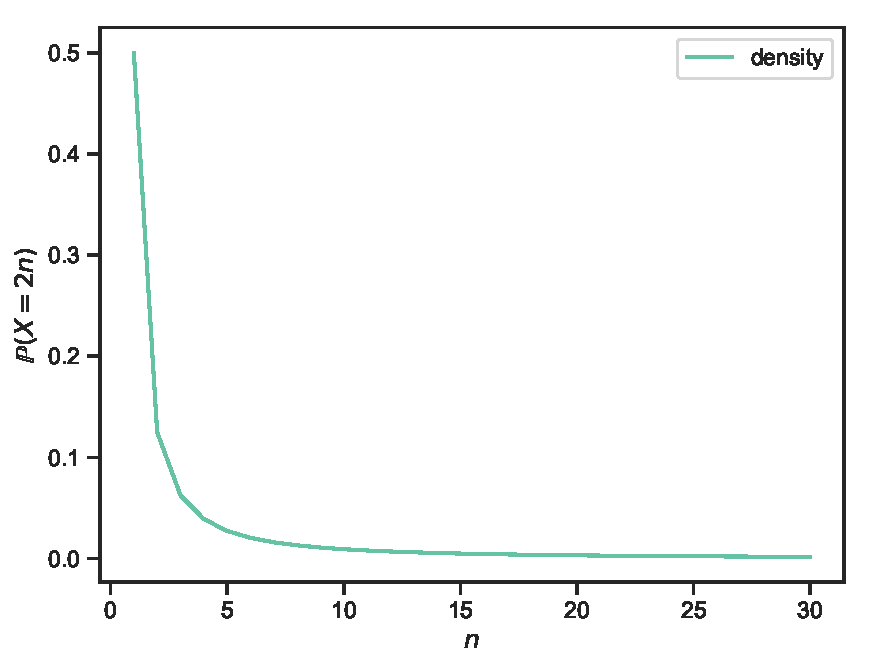
\includegraphics[scale=1]{../figures/X.pdf}
            \label{fig:density-X}
        \end{figure}

        Therefore, in our statistical test, we can compute the value of $X$ for the sequence $C(1), C(2), \dots$
        and check to see how it compares to the significance value $n = 128$ under the
        null hypothesis that the sequence $C(1), C(2), \dots$ has probability $p = \sfrac{1}{2}$ of success.
        If $X \geq 128$, then we know with at least $95\%$ confidence that the probability of success for $C$ must not have been $p = \sfrac{1}{2}$,
        and so the values in the sequence $x_1, x_2, \dots$ must be biased towards $[0, 0.5)$ or $[0.5, 1]$, instead of being uniformly distributed among the two intervals.

        This statistical test was implemented in the \texttt{X\_test.py} file and applied on the standard Mersenne Twister in Python.
        The test was performed $100$ times (using different seeds), and statistics regarding the tests are summarized in \autoref{tab:X}.
        As we can see, the Mersenne Twister was accepted $93\%$ of the time with a median value of $2$ and an average value well within the $95\%$ confidence interval.

        \begin{table}[H]
            \centering
            \caption{X Test Statistics}
            \begin{tabular}{|r|c|c|} \hline
                \multicolumn{1}{|r|}{Number of Acceptances} & \multicolumn{1}{|c|}{93}   \\ \hline
                \multicolumn{1}{|r|}{Number of Rejections}  & \multicolumn{1}{|c|}{7}    \\ \hline
                \multicolumn{1}{|r|}{Sample Average of X}   & \multicolumn{1}{|c|}{72.94}   \\ \hline
                \multicolumn{1}{|r|}{Sample Median of X}   & \multicolumn{1}{|c|}{2}   \\ \hline
            \end{tabular}
            \label{tab:X}
        \end{table}

        Therefore, the Mersenne Twister passes our test, and we can conclude that the Mersenne Twister sequence is,
        in the sense described above, uniformly distributed among the intervals $[0, 0.5)$ and $[0.5, 1]$.
\end{enumerate}
\end{document}
